\section{Material classes, core positions and future measurements}\label{sec:experiments}
We use the same three outcomes throughout. An \emph{excluded} hypothesis has a one-sided distance bound above the specified radius. A \emph{witness} is an actual material whose original field equations give a residual upper endpoint inside the ball. Anything else is \emph{unresolved}. Exclusion applies to the entire tested class. A witness proves existence. It can occur in several overlapping classes. Statistics below count independent materials separately from repeated measurements, widths and proof operations. All source choices use only the specified material prior and measurements already made.

\subsection{Amplitude and geometry under uncertain background}
A set of 24 independently generated pairs gives 48 base materials. Each is measured on four paired background realizations. Sixteen pairs share precisely the same nonzero cells and differ in amplitude. Eight share the same allowed region with different internal structures. To test both directions of the inverse question each material in a pair supplies data in turn and both candidate classes are tested. We determined the geometry families, parameter bands, noise and methods before generating the hidden materials. Sealed decisions precede comparisons with the generating arrays.

The controlled comparison uses 25 independent real cells on a square of side $0.70$ wavelengths, eight plane waves, twelve receiving directions over a half aperture and a $1.5\%$ joint complex noise level. Eight cells define the changing task region. Outside it the material is either known vacuum or free in $[0,b]$, with $b=1/32,1/16,1/8$. The background realization is paired between the two members of each amplitude pair. We use seven box half-widths, $0.5,0.9,1,1.5,2,3,5$ times a centre-dependent Neumann scale. The scale is the reciprocal of the reference feedback norm on the active cells in vacuum. Clipping enforces the material domain. The abscissa specifies the design; actual divergence is checked separately.

\begin{table}[tb]\centering
\caption{Decisions on 2688 data--class tests from 24 independent pairs. Cost is seconds summed over the common set. Search includes shared assembly when a method uses it. The second pair of cost columns distinguishes producing and independently checking a bound. Shared physical witness search and checking cost a further 21.7 s.}\label{tab:a}
\small
\begin{tabular}{@{}lrrrrrr@{}}\toprule
 & Excluded & Witness & Unresolved & Search & Bound & Replay\\\midrule
Directional perturbation &244&1488&956&1.65&59.50&3.70\\
Positive state form &925&1488&275&57.17&105.00&81.04\\
Indefinite state form &1116&1488&84&37.28&12.16&15.35\\
Fixed traces &1116&1488&84&26.87&3.61&12.56\\
Additional shared rows &1124&1488&76&2.30$^a$&38.21$^a$&0.08$^a$\\\bottomrule
\end{tabular}
\par\smallskip\parbox{.93\linewidth}{\footnotesize $^a$Increment over fixed traces. The reduced form also uses 6.50 s for the common base solves and about 0.20 s for the realisation of the multiplier bank. The same search limits and physical boxes apply to all five rows.}
\end{table}
The perturbation comparison uses \eqref{eq:neumann} with directional support of the linear term and an outward remainder. The positive-state comparison combines spatially independent multipliers and multiple source directions with separately chosen positive-state quadratic bounds. Positivity and the resulting sum of directional bounds are checked in the original coordinates. These are finite searches over specified multipliers and source frames. The numbers in table~\ref{tab:a} do not assert an optimum over all positive semidefinite dual representations. The full and reduced indefinite calculations use the same multiplier bank. The final row permits one, two, four or eight exact local material rows on cases that remain unresolved. A matched positive-state check used the complete positive source eigenspace, hence $\tr(H_+)$, for all 72 common weights at which $K\succ0$ could be verified. Across all 2688 tests it gave 1026 exclusions, 1488 witnesses and 174 unresolved. The search, proof and independent replay cost 34.16, 14.84 and 12.05 s in addition to the reference comparison. For the remaining 90 exclusions, all 6480 state matrices were checked. Of these 6446 had a strictly negative direction. For each of the remaining 34 positive states the positive-tail upper bound was below the noise threshold (maximum squared bound divided by squared radius 0.96439). The difference therefore holds throughout this finite weight bank.

All 1464 tests whose literal box contains the generating material retained it, including all 1344 generating paths. All 192 original measurements also admitted the generating material under independent full-wave checking, with residual upper endpoint below $0.999934r$. Of 1224 opposite-class boxes that did not contain that particular material, 32 had a different full-wave witness. For one same-profile pair at background cap $1/8$ and relative width three, data from a material of peak 3.87949 also admit a peak of 3.83695. The latter has residual at most 0.056287 against a radius of 0.060268. The active task-cell support agrees; the two legal backgrounds can differ. A procedure counting every opposite-class label as erroneous would misreport these genuine ambiguities. At the same weights the full and reduced forms agreed on every one of the 2688 decisions. Of their 1116 exclusions, 408 used a state block verified to be indefinite. In 119 distinct material boxes (192 data--box tests) an allowed perturbation had spectral radius greater than one.

\begin{figure}[tb]\centering
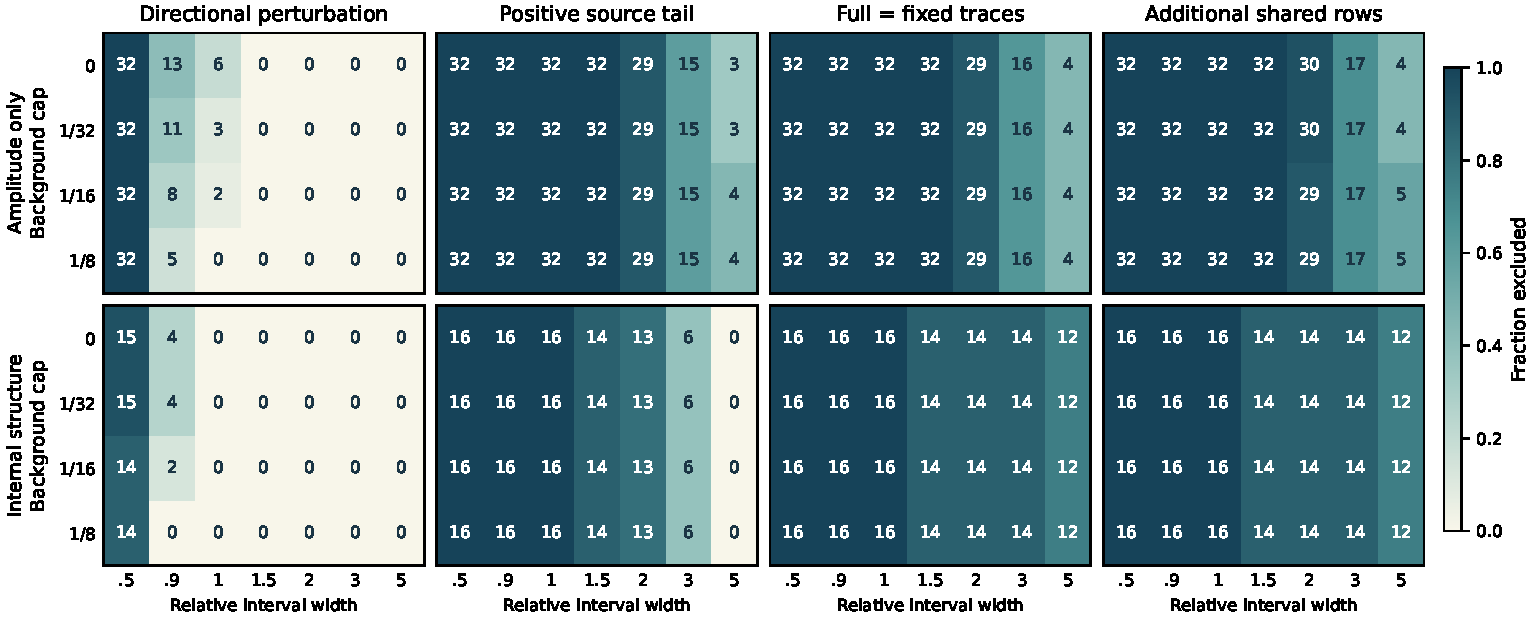
\includegraphics[width=.96\linewidth]{phase_comparison}
\caption{Exclusion over relative interval width and the allowed background. Each panel uses the stated physical hypothesis and shows the fraction of the opposite boxes outside the generating material which could be excluded. Methods and denominators refer to identical measurements in each comparison. Numbers are counts excluded. Positive-state comparisons include the full positive source tail. Full and fixed-trace tests agreed in every cell. Blank entries have no eligible boxes.}\label{fig:phase}
\end{figure}
Figure~\ref{fig:phase} distinguishes amplitude tests at identical support from changes of internal structure. A mechanism check explains the apparent gain from local realization: the eight additional exclusions arose in three amplitude pairs, and every successful local equation had interval $[0,0]$. Of 633 attempts, 388 selected at least one row with positive width. None of those attempts supplied an additional exclusion. An independent calculation that first set all known vacuum currents to zero and then applied ordinary full inertia reproduced all eight and gave twenty more. It left 56 hypotheses unresolved. The sharpness proposition therefore guides the interpretation: additional material information can help, but the results here favour exact use of known vacuum before refinement in unknown cells. The scalar rows remain a valid increasing hierarchy. For a separate cold-start convex comparison after the same vacuum elimination, we took both readings and both classes of all eight structural pairs at relative width three. The positive semidefinite search and the indefinite calculation each gave 14 exclusions and 18 witnesses on all 32 tests. The respective search and checking times were 198.88 and 0.209 s plus 0.327 and 0.017 s for independent checking (including the initial indefinite check in the latter 0.017 s). This comparison concerns the cost of attaining the same answers.

We also considered two larger physical controls at 400 MHz on a two-metre square, using 32 transmitters and 32 receivers. The native model has $96^2$ cells. Precisely 1153 are allowed to carry nonzero material. The measured low disk (peak 0.625) occupies 416 cells, and the hollow ring (peak 3.50) occupies 768. The competing solid profile uses all 1153. Its material can vary independently across these cells. The two calculations share a permitted active region; their actual supports differ. With $2\%$ error, the data distances to the competing class exceeded $1.7284r$ and $3.5945r$, respectively. The class widths were 5.14 and 3.09 times their reference contraction scales. For explicit permitted perturbations $\rho(wT)>1.0864$ and $>1.3896$, respectively. The halo outside the stated active region is known vacuum. The relative first Born error of the hollow ring is $376\%$.

The size of the search region materially changes this comparison. Figure~\ref{fig:scaling} shows 28 independent $96^2$ media on a two-metre domain ($ka=11.85$) and seven compact $24^2$ media. For the former, at $10\%$ noise the full-aperture Born class and nonlinear peak cap 0.5 were excluded on all 28, whereas the chosen bounds excluded cap 0.75 on none. For the compact set the joint bound excluded cap five on five of seven and the material of peak 4.28 supplies a physically legal control. These are distinct data and material contracts. The compact comparison has $ka=4.27$, twelve incident fields, 48 receiving ports and $1\%$ noise; the large-domain comparison has ten fields and 20 ports. Here $a$ is the enclosing radius of the computational square. The numbers identify a limitation of unrestricted peak inference in one aperture and electrical size. They do not define a geometry-independent limiting contrast. The angular bandwidth of radiated fields is itself a scale, not a strict finite rank \cite{bucci87}.
\begin{figure}[tb]\centering
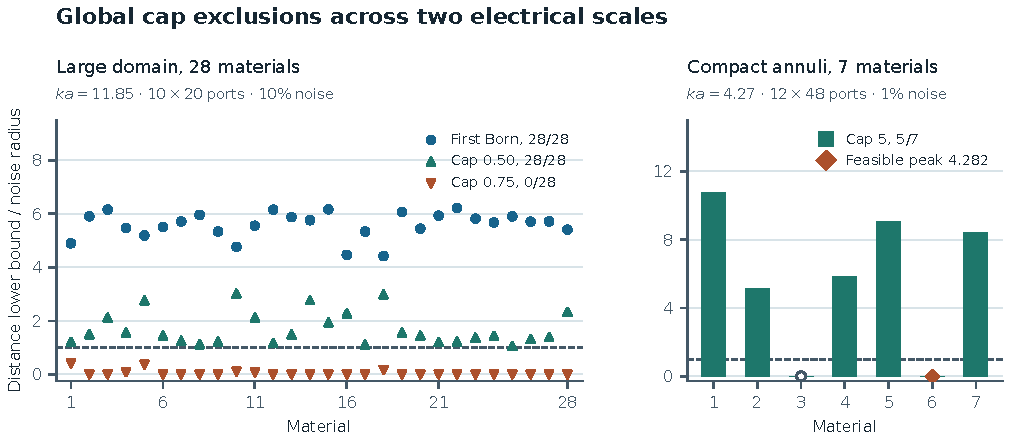
\includegraphics[width=.93\linewidth]{scaling}
\caption{Independent materials at two electrical sizes. A point above one excludes the stated hypothesis. A point at or below one measures the limit of the calculation. In the right panel one material is known to be within the proposed cap. Material indices are local to each panel.}\label{fig:scaling}
\end{figure}

\subsection{Mapping a core without an initial image}
We next tested the question a map answers. On a $12^2$ grid there were seven transmitted beams and nine receiving ports on arcs, at 135 MHz on a two-metre square. The noise radius was $3\%$, with a small allowance for forward arithmetic. We generated three independent objects, a disk, two inclusions and an annulus. Inside the mandatory core each cell could vary in $[0.75,1.375]$, in the outer layer in $[0,1.375]$, and in the background in $[0,b]$. The paired and annular templates preserve their stated separation and cavity. The unknowns included every permitted material value and the discrete centre in the pictured search window. The centre tree started from the whole window.

\begin{figure}[tb]\centering
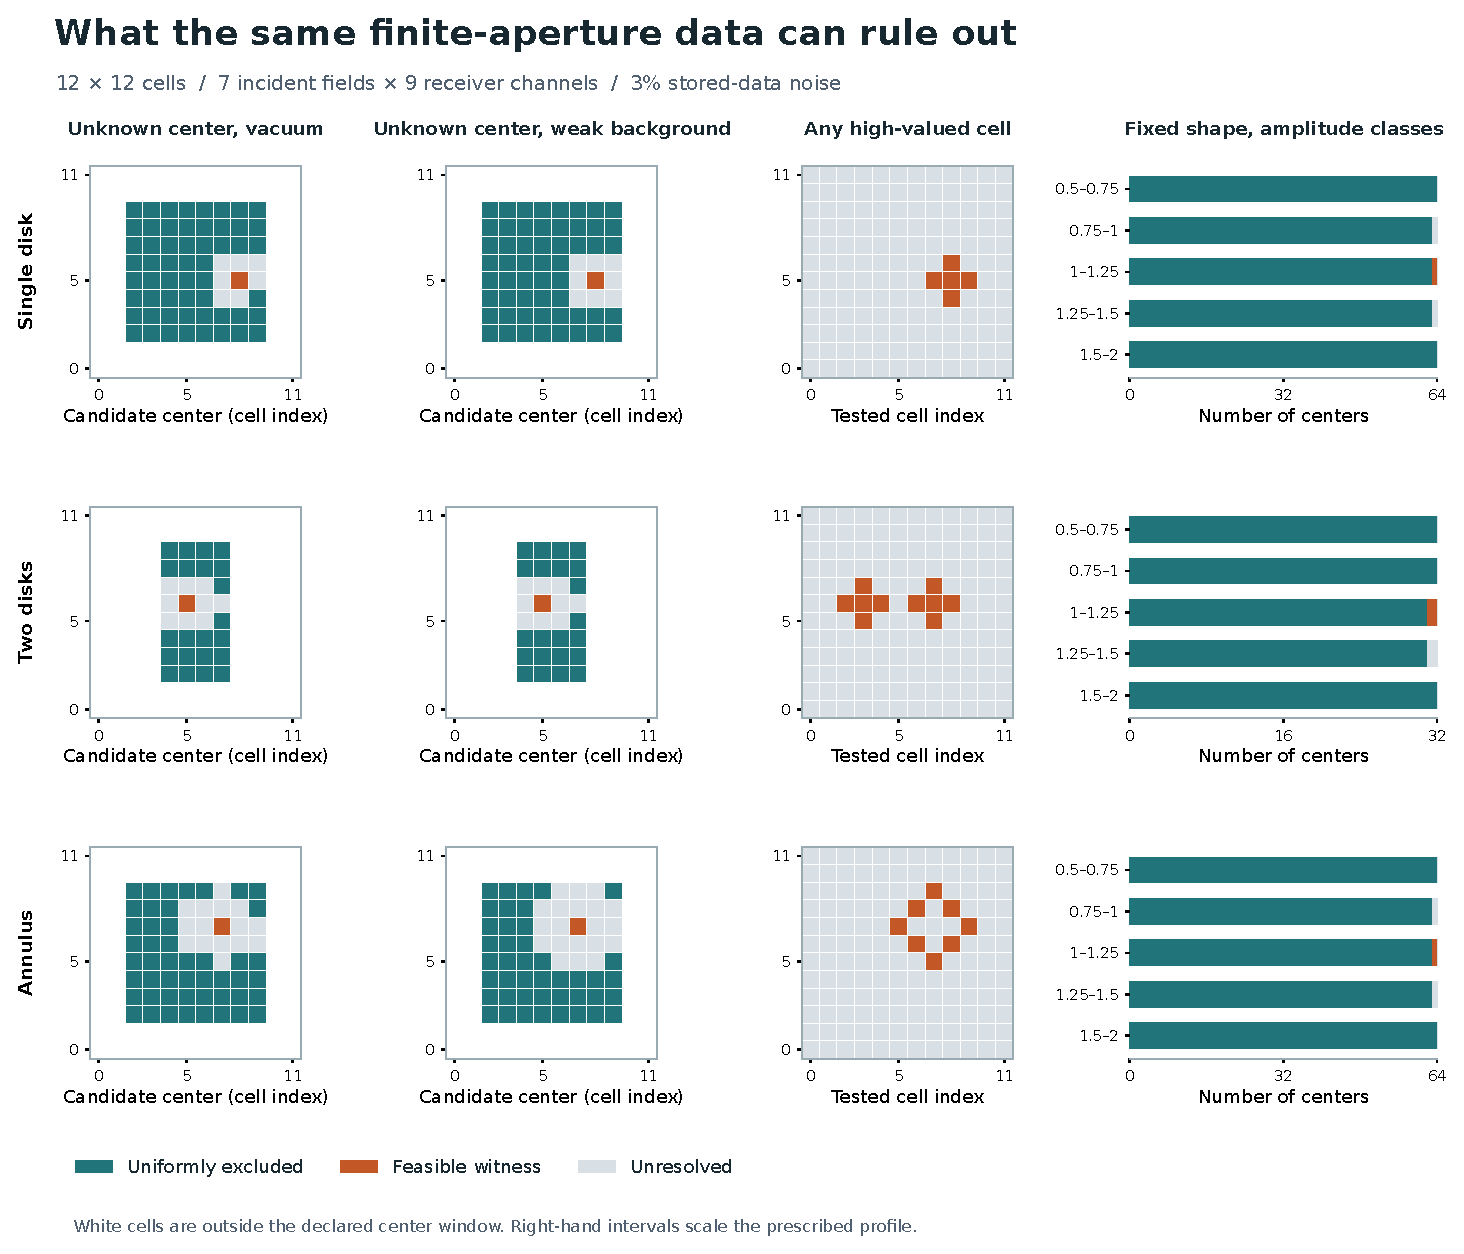
\includegraphics[width=.95\linewidth]{spatial-map}
\caption{Spatial hypotheses tested against the same complex readings. Centre maps ask where a specified finite core can occur; the single-cell query allows arbitrary material elsewhere. A compatible label requires an actual forward solution. Remaining labels may still be impossible.}\label{fig:map}
\end{figure}
With $b=1/32$, the numbers of excluded, compatible and unresolved centres were $(55,1,8)$ out of 64 for the disk, $(22,1,9)$ out of 32 for the two inclusions and $(43,1,20)$ out of 64 for the annulus. Setting $b=0$ raised the exclusion counts to 56, 22 and 48. Each material was also tested under a stated shape profile with five possible amplitude intervals. All three admitted a witness in $[1,1.25]$. The surviving interval hull was $[0.75,1.5]$ for the disk and ring and $[1,1.5]$ for the two inclusions. In contrast, on permitting all other cells to range freely in $[0,1.375]$, none of 432 propositions that a specified cell could reach one was ruled out. Twenty-three had witnesses (figure~\ref{fig:map}).

A separate $96^2$ experiment used seven transmitters and nine receivers drawn from the finite native arcs at 400 MHz, a $4\%$ error radius and a core of radius two cells, outer radius three and a vacuum exterior. On a $16$ by $16$ centre grid, 247 centres were excluded, one had an explicit witness with residual below $0.980r$, and eight remained unresolved. The computation descended through 21 parents whose allowed outer regions were too large for the chosen direct test. All 70 excluding nodes were checked against the original Fourier kernel. The result covers all 256 centres in this window even though many material coordinates were never subdivided.

\begin{figure}[tb]\centering
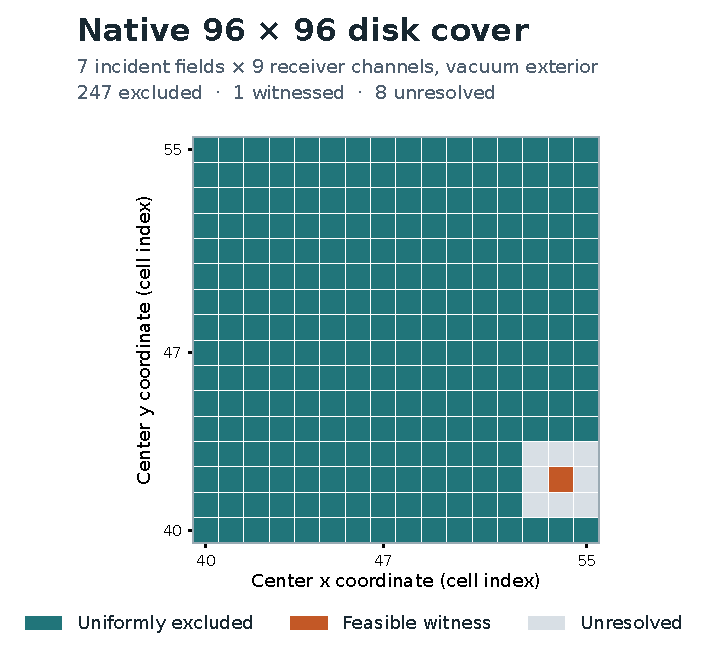
\includegraphics[width=.82\linewidth]{native-center-map}
\caption{Core position on the native grid. The seven transmitting angles run from $-67.5$ to $67.5$ degrees and the nine receiving angles from $-78.75$ to $67.5$ degrees. The result applies to an independently varying core and layer with the stated minimum thickness. The true material is used only for evaluation.}\label{fig:nativemap}
\end{figure}
A separate moving-support implementation used 100 and 1000 different boxes on 53 and 64 distinct nine-cell supports, respectively. The common state block was positive definite and each local update invertible. Precomputing the full trace Gram once allowed a small submatrix to be gathered for each support. A second bordered elimination with $-D_\theta^{-1}$ reduced the order from 151 to 25. These timings apply to this more restrictive moving-support algorithm; the fixed-row, singular-safe comparison of theorem~\ref{th:fixed} is the preceding 2688-box study. The machine-precision checks took 0.595 and 5.909 s in full coordinates, versus 0.018 and 0.154 s after reduction, with identical signs in every box. The reduced 128-bit computation for all boxes took 0.224 and 2.817 s after 0.598 and 0.736 s of cold preparation. Model construction, loading and box generation together took at most 0.046 s. Full-matrix interval rechecks of 16 and 32 boxes took 4.392 and 10.390 s. The strict decisions excluded 97 of 100 and 985 of 1000. These are distinct production and replay costs. The smaller floating-point times alone would overstate the end-to-end benefit.

\subsection{Can prospective illumination reduce the set?}
We tested the conditional operator on six independent synthetic media, two per geometry. All three arrays had three receivers. The first had unequal radii and asymmetric angles, the second used a $130$ degree arc, and the third kept three ports of a masked array. Masking a port did not insert a scattering obstacle. The square was $0.70$ wavelengths wide at 400 MHz, with a $4$ by $4$ discretization. For each object the task prior consisted of two competing interval material classes. Public nominal centres with near-equal old responses were prepared independently of the generating material, which was drawn within one class. Both nominal centres gave strictly compatible old full-wave fields in all 24 class--energy conditions in each of the following two comparisons.

We initially illuminated at $0$ and $180$ degrees. From ten further angles at $30$ degree spacing we selected batches of one, two or four, giving 10, 45 or 210 possible actions. In the added-energy regime each beam had unit incident fluence. In the fixed-total regime the two old beams were acquired separately at half energy each and one further unit was shared among the new beams. Noise was an absolute bound per receiving column. Each method had the same angular menu and the same post-acquisition tests. Random choice, uniform angular completion, a local nuisance-adjusted Fisher design and \eqref{eq:gap} were compared. Each proposal and its receiving direction were stored before calling the separate future-measurement program. After acquisition the stored support test was applied before repeating the joint inertia test.

At half-width $0.0008$ and absolute per-beam radius $0.00018$, all 3180 candidate actions across materials, energies and batch sizes had a strictly positive gap. Each policy removed the incorrect class on the first beam in all six media for both energy budgets. This establishes causality of the prospective calculation, but the menu was too easy to distinguish angular policies. We repeated the same media with four times the width and a radius of $2\%$ of the old added-energy RMS column norm. The rule was chosen before collecting the new readings for this comparison. It changes both width and noise, and adds no independent objects.

\begin{table}[tb]\centering
\caption{Number of the six media for which the selected batch provably separates the two classes before acquisition in the larger intervals. The last block gives wrong-class removals with the realized data. The three columns of each block correspond to one, two and four additional beams.}\label{tab:active}
\small\begin{tabular}{@{}lccc@{}}\toprule
Selection & Added fluence & Fixed total & Fixed total, realized\\\midrule
Random &5,5,6&3,3,3&6,5,6\\
Uniform angle &6,6,6&6,5,4&6,6,6\\
Nuisance-adjusted Fisher &6,6,6&5,5,3&6,6,6\\
Conditional response &6,6,6&6,6,4&6,6,6\\\bottomrule
\end{tabular}
\end{table}
In this comparison, 2016 of 3180 actions had a proven edge for the specified bounds. Only 345 of 1260 four-beam fixed-total actions did so. The four-beam menu had no proven edge for two of the six objects. Splitting a fixed energy among beams while keeping the absolute error per beam fixed can reduce guaranteed separation. The conditional choice increased the median one-beam support margin from 0.00765 for uniform completion to 0.01891. In both cases all six realized first beams sufficed. Of 144 realized paths, 143 removed the incorrect class; the saved support alone did so in all 143 and the joint update alone in 140. The remaining path was a random two-beam choice under fixed total energy. All 144 true material witnesses survived. These results concern the two stated priors, not all material images.

\begin{figure}[tb]\centering
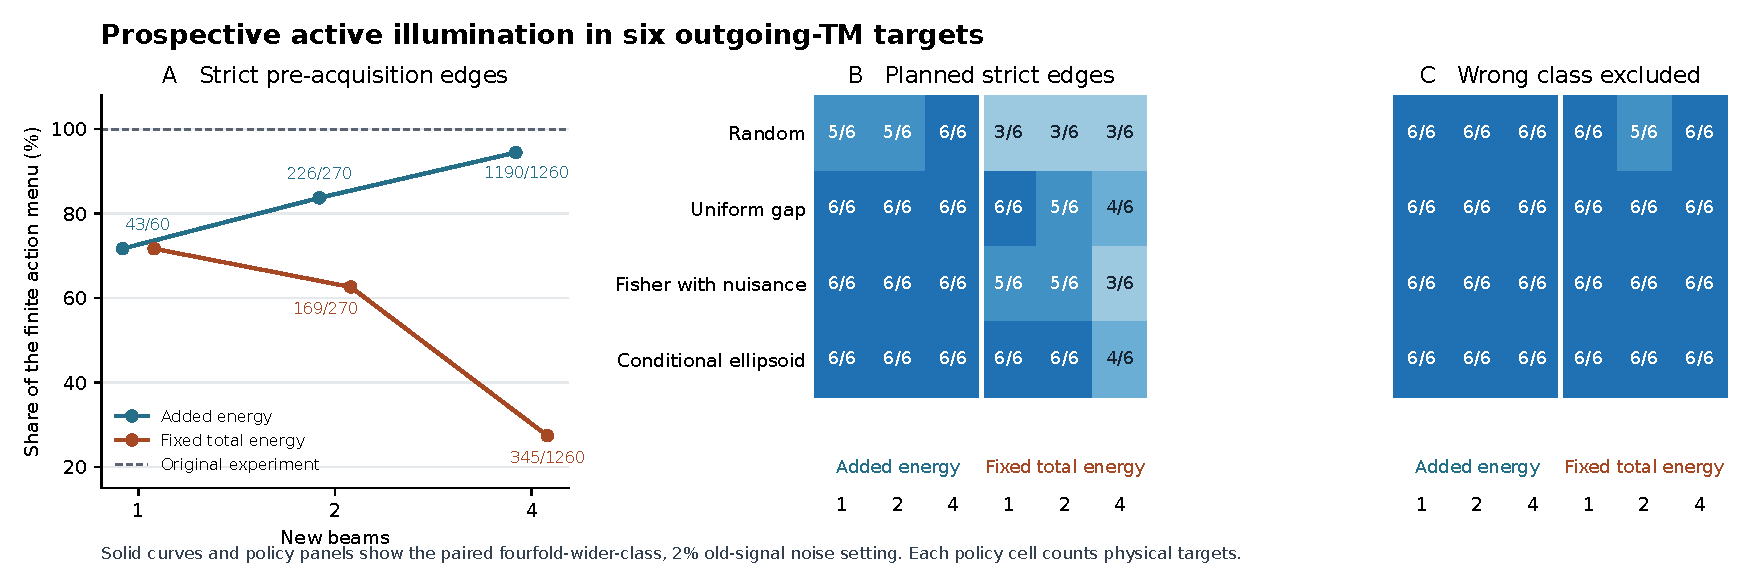
\includegraphics[width=.92\linewidth]{active_policy}
\caption{Prospective separation under different allocations of the same incident energy. Each line or cell summarizes the same six physical media. Success after observing a favourable reading can occur even when the old data provide no worst-case separation guarantee.}\label{fig:active}
\end{figure}
The positive-state weights on these narrow classes saturated and had a positive receiving block in all 192 weight tests in each comparison. All 96 broad indefinite trials on $[0,3]^{16}$ per comparison had an old index deficit. Thus the compact prospective demonstration uses positive-state weights. The frozen receive direction joined the predicted centres, with the joint Frobenius noise allowance applied to batches of columns. The four-beam shortfall is therefore specific to that direction, energy split and noise envelope. An old-data receiver-space cone optimization on all 120 single-beam choices of the sensitivity study improved each of the 86 positive margins, while the same 86 choices remained separated. The other 34 supplied no strict separation in either calculation.

A further test used the same two occupied classes of each compact object and the same old readings, with positive sector weights and a signed optical multiplier on one cell. Both class forms in all six objects had $\nu=k_o=1$ and a positive receiving square under the added-energy convention. For each of the 60 single-beam choices an interval-verified point on the line of their centres belonged to both clean response ellipsoids. No receive direction separates those two outer sets, even at zero future noise. The positive-state forms in the original experiment already separate the classes. This provides a full-wave indefinite example and isolates a genuine loss in the chosen outer bounds.

A separate native computation tests whether saturation and receiving positivity can fail independently. It uses the disk and hollow ring readings in the $1153$-cell active region, three fixed material forms, and prefixes of 1, 2, 4, 8, 16 and 32 old beams. The original full noise majorant is kept for every prefix as a conservative choice. Prediction from \eqref{eq:index} and direct interval inertia of the $32$ by $32$ receiving block agree on all 36 cases. In the solid class of half-width $2.5$, the disk data saturate with 16 and 32 beams ($k_o=\nu=13$), yet the receiving block has 25 positive and seven negative directions. At 32 beams the ring gives the same source-side deficit of seven, with $k_o=6$ and 32 positive receiving directions. Neither calculation gives the bounded conditional operator of theorem~\ref{th:response}. These prefix tests diagnose a fixed form; they do not establish old-data compatibility of a rival class.

A nonempty native example removes this last ambiguity. We acquired two synthetic beam readings from the centre of the solid class of half-width 1.5, keeping the same receiver, material form and error bound $r=0.0388901$. The resulting 64 complex values reproduce the complete two-beam forward solution to within $4.08\times10^{-17}$. Since $K\succ0$, the strict data slack makes $\Po\prec0$. Saturation here is automatic for compatible data at a positive definite state block. The material-only state has eleven negative directions, the old source pivot has two positive directions, and the receiving block has exactly 23 positive and nine negative directions. Here the shortage follows already from having two old beams for eleven material modes. This example establishes occupancy on the native grid. Its freely varying receiving square is indefinite even with arbitrarily accurate readings inside the stated error contract. Figure~\ref{fig:source} shows how this possibility arises.

\begin{figure}[tb]\centering
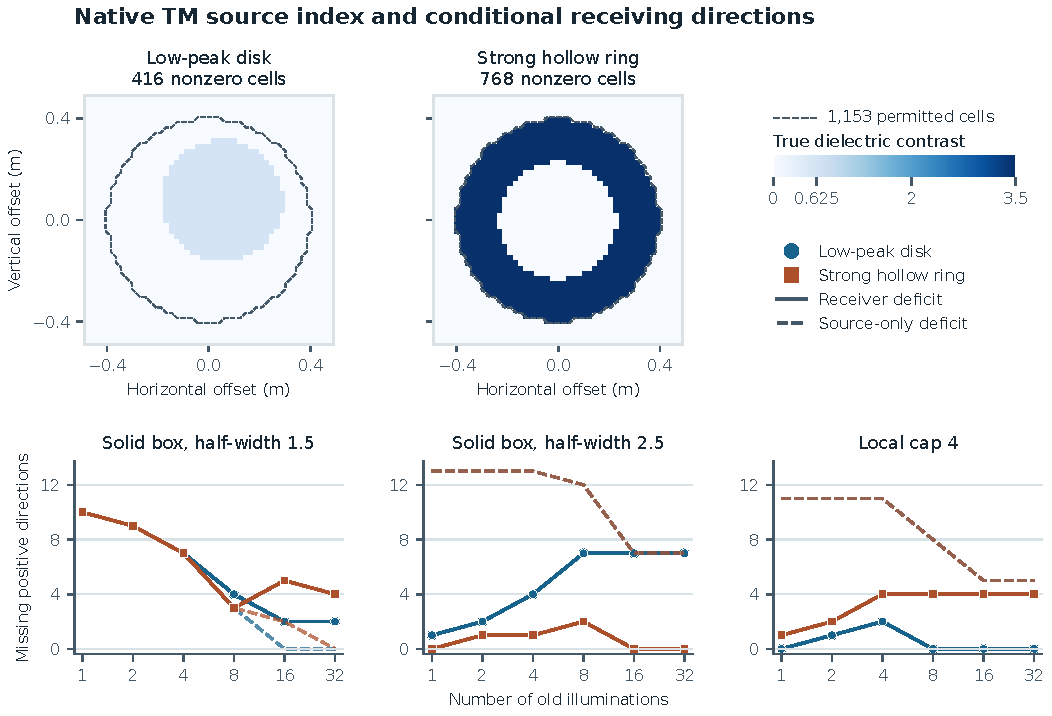
\includegraphics[width=.93\linewidth]{native-source-index}
\caption{Two measured materials within the same permitted region, and the two distinct index conditions. The dashed curves show the source-side deficit; solid markers show the number of missing positive receiver directions obtained by independent interval evaluation. The original noise radius for each object is used at every source count.}\label{fig:source}
\end{figure}
For the tighter solid interval, the 32 incident fields have eleven positive generalized source directions, exactly the number required by corollary~\ref{cor:energy}. In units of the incident intensity of one original beam summed over the full square, the infimum in \eqref{eq:energy} is in $[0.59082793,0.59082795]$ at the disk error radius and $[3.74429999,3.74430008]$ at the ring radius. The wider solid interval has thirteen negative material directions and only six positive dictionary directions. The corresponding uniform cap of four has eleven and six. Unlimited fluence in the same dictionary therefore leaves deficits of at least seven and five, respectively. This statement is independent of a particular old receiving record and is specific to its fixed spatial weight. No feed-network power calibration is assumed.

We tested this energy threshold with an occupied class (figure~\ref{fig:nativebeam}). Fix eleven exposures, the same per-column error allowance $r/\sqrt{11}$, and exactly $1.25 E_{\rm inf}$ incident fluence ($0.738535$ in these units). The plane-wave design takes eleven separated dictionary angles; the coherent design uses the leading generalized eigenbeams. Both see the same solid material, the same port geometry and the same normalized noise realization. Saturation holds for both. The coherent design makes $R_y$ positive definite ($\lambda_{\min}>0.00266$), while the angular design leaves five negative receiving directions. This is a strict difference in bounded prediction under one material form at equal incident energy.

The wider solid class was also tested with a physical material in its interior. With 16 and 32 ordinary beams, $\nu=k_o=13$ in both cases; direct evaluation gives 25 positive and seven negative receiving directions in both. This example has enough sources by count and a strictly compatible full-wave solution. Its deficit is the shortage of positive dictionary directions in \eqref{eq:indexsmall}. The narrower and wider tests shared one simultaneous 32-right-hand-side physical solve. Including validated spectral and receiving calculations, the narrow comparison took 78.75 s and the additional wide comparison 38.10 s.

\begin{figure}[tb]\centering
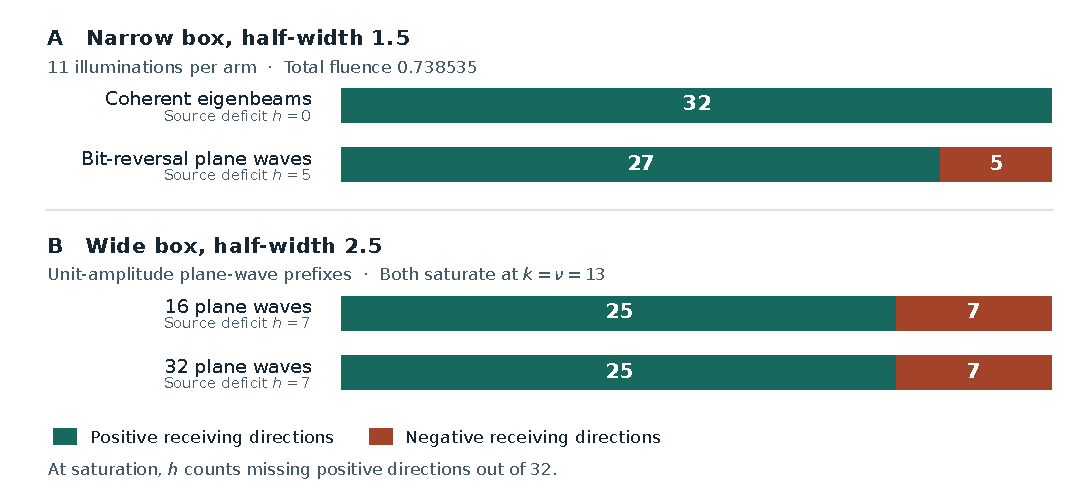
\includegraphics[width=.91\linewidth]{native-illumination}
\caption{Receiving directions on an occupied native material class. Left, identical fluence and eleven exposures per design. Right, nested ordinary-angle prefixes for the wider interval. In both panels a nonpositive receiving direction is a limit of the chosen bound on the scattered response.}\label{fig:nativebeam}
\end{figure}


\subsection{Model errors and microwave measurements}
Synthetic results above come with two distinct numerical error specifications. For the broad comparison the stored discrete matrices are the defined operator. For the compact prospective study the interval evaluation includes the equal-area disk and Hankel cell model itself. Both differ from a bound on replacing a physical continuum by that model. On one aligned square inclusion, evaluation of the discrete kernels on $8^2$ and $16^2$ grids enclosed the relative field difference between 0.04600043134948238 and 0.04600043134948240. On six other media compared on $96^2$ and $32^2$ at full and half aperture, individual differences ranged from $12.43\%$ to $35.43\%$. This is a sample discrepancy, not a uniform correction for all media in the class.

For a calibrated measurement $Y=(I+\Delta)F+\eta$ with $\|\Delta\|\le\epsilon<1$ and $\|\eta\|_F\le r_\eta$, the clean distance obeys
\begin{equation}
 \|F-Y\|_F\le(\epsilon\|Y\|_F+r_\eta)/(1-\epsilon).
 \label{eq:gain}
\end{equation}
Indeed $\|F-Y\|_F\le\epsilon(\|Y\|_F+\|F-Y\|_F)+r_\eta$. For common gain error $\mathrm i/32$ and additive error $1/2048$, interval arithmetic bounded the realized error by 0.016397 and the data-dependent upper bound by 0.017657.

We applied the error accounting to the Fresnel and Manitoba microwave data \cite{fresnel,manitoba}. There are seven physical specimens. The three Fresnel targets contribute nine target--frequency pairs at 4, 6 and 8 GHz. Four Manitoba targets contribute 28 pairs at 3--6 GHz. The nonnegative Born distance exceeded the empty-field reference error on three and 25 pairs, respectively. Relative errors on unused receivers ranged from $80.2$ to $97.9\%$ and from $68.1$ to $107.9\%$. The nonlinear contrast limit of one for the large nylon cylinder at 3 GHz had a remaining margin of $4.018\%$ of the measured norm beyond the reference allowance. It would exclude that material hypothesis only if the total additional loaded-system discrepancy were smaller than this margin. No uniform loaded discrepancy of that size was established.
